\documentclass[10pt,a4paper]{amsart}
\usepackage[margin=19mm]{geometry}
\usepackage{amsmath,amssymb,mathtools}
\usepackage[scr=rsfs,cal=euler]{mathalfa}
\usepackage{xfrac}
\usepackage[unicode,hidelinks,bookmarks=false]{hyperref}
\newcommand{\ie}{i.e.\ }
\newcommand{\cf}{cf.\ }
\newcommand{\resp}{respectively\ }
\newcommand{\Subsection}{\subsection}
\providecommand{\nobreakdash}{\nobreak\hbox{-}}
\setlength{\emergencystretch}{2em}
\multlinegap0pt
\usepackage{tikz}
\usepackage{xcolor}
\usepackage{amssymb}
\newtheorem{theorem}{Theorem}
\newtheorem{example}{Example}
\newtheorem{proposition}{Proposition}
\title{On subgroups of Brin-Thompson groups $nV$}
\author{Sadayoshi Kojima, Xiaobing Sheng}
\date{Source: arXiv:2603.18410v3 (CC BY 4.0)}
\begin{document}
\maketitle

\noindent\emph{Source and licence.} On subgroups of Brin-Thompson groups $nV$. Version arXiv:2603.18410v3 (CC BY 4.0), distributed by arXiv under the Creative Commons Attribution 4.0 International licence, http://creativecommons.org/licenses/by/4.0/, as recorded in the arXiv licence metadata for this exact version and shown on the abstract page https://arxiv.org/abs/2603.18410v3. Full licence notice: \texttt{licenses/arxiv-2603.18410-CC-BY-4.0.txt}.\par\smallskip

\noindent\textit{Editorial scope.} Counted unit: the article's proposition Prop:QEmbeds2V (source0.tex lines 1720--1722). The article's complete original proof of it is delivered with it (source0.tex lines 1723--1814, one \texttt{proof} environment of 92 lines). No mathematics is written, repaired or re-derived: the statement and the proof are the article's own lines, in the article's own notation, and no retained line is substituted or re-flowed.  Retained uncounted as the source-local context the proof needs: lines 154--164; lines 1439--1521.  One declared adaptation: exactly 1 ancillary strings inside the retained spans are omitted (image-inclusion commands and, where the source repeats a label, the repeated label definitions) and no other line differs from the source; the figure environments, with their placement, captions and labels, are kept, and the package records the omitted strings in fidelity receipts bound to the affected bodies.  No retained line contains a citation, so the wrapper carries no bibliography and no bibliography entry.  The retained lines contain the article's own diagram code, which the wrapper typesets with the standard tikz packages; no image file is delivered and the package declares no asset dependency.  Editorial formatting only, in addition: an AMS \texttt{amsart} preamble that restates the article's own declarations and macros used by the retained lines, namely the environments \texttt{theorem}, \texttt{example}, \texttt{proposition} on separate counters, together with the standard packages those lines need.  The retained environments print in this document as Theorem 1, Example 1, Proposition 1 in order of appearance, whereas the article prints the same items with the numbering of its own full document.  The complete native source of the article as distributed in the arXiv e-print for this exact version is bundled unchanged as \texttt{sources/196693/source0.tex}.
\begin{theorem}\label{Thm:Main2} 
        For $n \geq 2$,  
	then the Brin-Thompson group  $nV$  contains continuum many copies of
	the additive group of the rationals  $\mathbb{Q}$  sharing 
	the subgroup isomorphic to  $\mathbb{Z}$.  
% 	$nV$  contains a subgroup isomorphic to 
%	an additive group of the dyadic rationals if  $n \geq 2$, 
%	and in particular, 
%	\textcolor{red}{$nV$} contains elements of infinite order having roots with arbitrarily 
%	large order.  
\end{theorem} 

\begin{example}\label{Ex:Root} 
	We start with an infinite order element  $h$  
	as depicted on the 
	right
	of Figure \ref{Fig:Root}
	which is represented by  $(S, T)$ with a labeling in each subblock.  
	The induced vertical permutation by  $h$  is the identity, 
	namely the subblock labelled by  
	$*$
	in  $S$  is mapped to the subblock 
	$*$
	%}   
	in   $T$.     
	A root  $h_1$  of  $h$  of order  $2$  is 
        depicted on the 
        right
        of Figure \ref{Fig:Root} as  $(S_1, T_1)$.   
	\begin{figure}[htp]
		\begin{center} 	      
		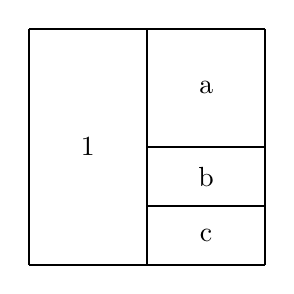
\begin{tikzpicture}[baseline=-0.65ex, thick, scale=0.3]
                 \draw (0, -5) to (0,5);
                 \draw (0, -5) to (10, -5);
                 \draw (10, -5) to (10,5);
                 \draw (10, 5) to (0, 5);
                 \draw (5, -5) to (5,5);
                 \draw (5, -2.5) to (10,-2.5);
                 \draw (5, 0) to (10,0);
                 \draw (2.5, 0) node{1};
                 \draw (7.5, 2.5) node{a};
                 \draw (7.5, -1.25) node{b};
                 \draw (7.5, -3.75) node{c};
         \end{tikzpicture}
         \begin{tikzpicture}[baseline=-0.65ex, thick, scale=0.3]
                 \draw (5, 0) node{$\mapsto$};
                 \draw (5, -7) node{$h_1$};
                 \end{tikzpicture}
         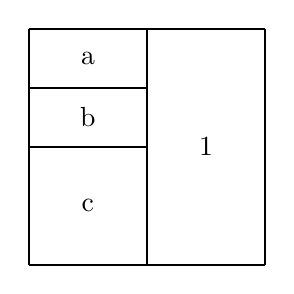
\begin{tikzpicture}[baseline=-0.65ex, thick, scale=0.3]
                 \draw (0, -5) to (0,5);
                 \draw (0, -5) to (10, -5);
                 \draw (10, -5) to (10,5);
                 \draw (10, 5) to (0, 5);
                 \draw (5, -5) to (5,5);
                 \draw (5, -5) to (5,5);
                 \draw (0, 2.5) to (5,2.5);
                 \draw (0, 0) to (5,0);
                 \draw (2.5, 3.75) node{a};
                 \draw (2.5, 1.25) node{b};
                 \draw (2.5, -2.5) node{c};
                 \draw (7.5, 0) node{1};
        \end{tikzpicture}
                 \quad
        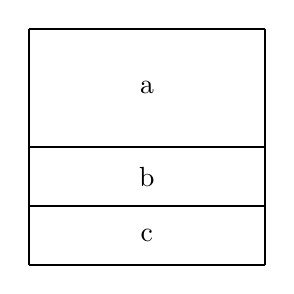
\begin{tikzpicture}[baseline=-0.65ex, thick, scale=0.3]
                 \draw (0, -5) to (0,5);
                 \draw (0, -5) to (10, -5);
                 \draw (10, -5) to (10,5);
                 \draw (10, 5) to (0, 5);
                 \draw (0, 0) to (10,0);
                 \draw (0,-2.5) to (10, -2.5);
                 \draw (5, 2.5) node{a};
                 \draw (5, -1.25) node{b};
                 \draw (5, -3.75) node{c};
        \end{tikzpicture}
        \begin{tikzpicture}[baseline=-0.65ex, thick, scale=0.3]
                 \draw (5, -7) node{$h$};
                 \draw (5, 0) node{$\mapsto$};
                 \end{tikzpicture}	
        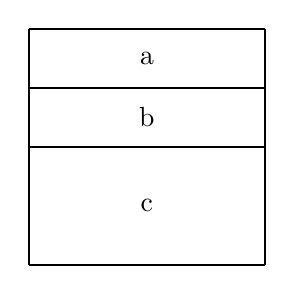
\begin{tikzpicture}[baseline=-0.65ex, thick, scale=0.3]
                 \draw (0, -5) to (0,5);
                 \draw (0, -5) to (10, -5);
                 \draw (10, -5) to (10,5);
                 \draw (10, 5) to (0, 5);
                 \draw (0, 0) to (10,0);
                 \draw (0,2.5) to (10, 2.5);
                 \draw (5, 3.75) node{a};
                 \draw (5, 1.25) node{b};
                 \draw (5, -2.5) node{c};               
        \end{tikzpicture}
                    %  	
                 	\caption{$h$  and its root  $h_1$  of order  $2$}
			\label{Fig:Root}
		\end{center} 	
	\end{figure} 
\end{example} 

\begin{proposition}\label{Prop:QEmbeds2V}
       The group $nV$  contains a subgroup isomorphic to  $\mathbb{Q}$ for $n \geq 2 $.
\end{proposition}

\begin{proof} 
         Since there is an obvious sequence of isomorphic embeddings of 
         Brin-Thompson groups  $2V < 3V < \cdots$, 
         we only need to prove Theorem  \ref{Thm:Main2}  for  $n = 2$. 
 	Next, we construct a sequence of groups in $2V$
	\begin{equation}\label{Eq:seq} 
		\langle s_1 \rangle  <  \langle s_2 \rangle  < \cdots <  \langle s_k \rangle 
	\end{equation}
	generated by roots of  $h$  of order $k!$.
	Here we take $s_1 = h$ and $s_2 = h_1$ 
	as constructed in Figure \ref{Fig:Root}.
	We then construct $s_3$ as follows.   
	Start with a block in the form of  $L_2$, 
	then we embed  $L_3$  into each subblock of $L_2$  with horizontal scaling 
	and we denote it by $L_{2,3}$.  
	The product of the numbers in the tuples in the suffix 
	indicates the number of vertical blocks  $3\cdot 2 = 3!$.  
	Then, 
	we let  $s_3$  be generate by a horizontal slide with  
	a ``vertical shifting" at the central vertical line
	as depicted in Figure \ref{Fig:jthRoot}.
 	\begin{figure}[htp]
		\begin{center}
          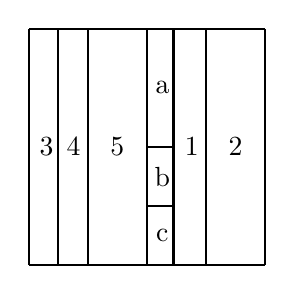
\begin{tikzpicture}[baseline=-0.65ex, thick, scale=0.3]	
		  \draw (0, -5) to (0,5);
                 \draw (0, -5) to (10, -5);
                 \draw (10, -5) to (10,5);
                 \draw (10, 5) to (0, 5);               
                 \draw (5, -5) to (5,5);
                 \draw (1.25, -5) to (1.25,5); 
                 \draw (2.5, -5) to (2.5,5); 
                 \draw (5, -2.5) to (6.125,-2.5);
                 \draw (5, 0) to (6.125,0);             
                 \draw (6.125, -5) to (6.125,5);    
                 \draw (7.5, -5) to (7.5,5);        
                   
                 \draw (5.65, 2.5) node{a};
                 \draw (5.65, -1.25) node{b};
                 \draw (5.65, -3.75) node{c};   
                 
                 \draw (0.75, 0) node{3};
                 \draw (1.9, 0) node{4};
                 \draw (3.75, 0) node{5};   
                 \draw (6.9, 0) node{1};   
                 \draw (8.75, 0) node{2};   
           \end{tikzpicture}
           \begin{tikzpicture}[baseline=-0.65ex, thick, scale=0.3]
                 \draw (5, -7) node{$s_{3}$};
                 \draw (5, 0) node{$\mapsto$};
                 \end{tikzpicture}	
                 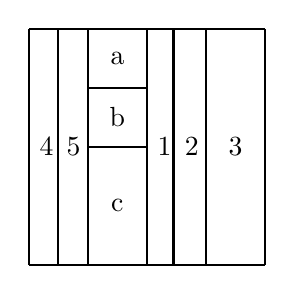
\begin{tikzpicture}[baseline=-0.65ex, thick, scale=0.3]
               \draw (0, -5) to (0,5);
                 \draw (0, -5) to (10, -5);
                 \draw (10, -5) to (10,5);
                 \draw (10, 5) to (0, 5);               
                 \draw (5, -5) to (5,5);
                 \draw (1.25, -5) to (1.25,5); 
                 \draw (2.5, -5) to (2.5,5);          
                 \draw (6.125, -5) to (6.125,5);    
                 \draw (7.5, -5) to (7.5,5);      
               
                 \draw (2.5, 0) to (5,0);
                 \draw (2.5,2.5) to (5, 2.5);
                 \draw (3.75, 3.75) node{a};
                 \draw (3.75, 1.25) node{b};
                 \draw (3.75, -2.5) node{c};      
                  
                  \draw (0.75, 0) node{4};
                 \draw (1.9, 0) node{5};
                 \draw (5.75, 0) node{1};   
                 \draw (6.9, 0) node{2};   
                 \draw (8.75, 0) node{3};        
                 \end{tikzpicture}
			\caption{The root  $s_3$  of  $s_2$  of order  $3$}
			\label{Fig:jthRoot}
		\end{center} 	
    	\end{figure} 
	
	Finally,  
	by repeating the construction of the block pairs $L_{1,2, \cdots, k}$,  
	we obtain a sequence of elements  $s_k \in 2V$ 
	so that each generates a finite cyclic group 
	which contains the ones generated by the previous elements in the sequence
	and in particular  $\langle s_k \rangle$  can be embedded in  $\mathbb{Q}$.
	Thus, 
	we have the following inductive limit 
	\begin{equation*} 
		\bigcup_{k = 1}^{\infty} \, \langle s_k \rangle 
	\end{equation*}
 	that contains a root of  $h$  of arbitrary order and hence    
	is isomorphic to  $\mathbb{Q}$.  
\end{proof}

\end{document}
